Uma série temporal é uma coleção de observações $x_t$ registrada no tempo $t$.
Esse tempo pode ser discreto ou contínuo. Na nossa análise, o tempo é contínuo,
entretanto, interpretamos ele como discreto, já que as medições são guardadas a
cada hora. O objetivo de analisar a série temporal é tentar compactar a
informação disponibilizada pela prefeitura para interpretação a posteriori,
estudar a relação com outras variáveis medidas e prever futuros valores usando
algum modelo. Nesse caso, mostraremos mais de um. Observe a série temporal de
Ozônio no ano de 2018 na Figura \ref{time-series}. Grande parte desse texto
também é contido no livro Econometria de Séries Temporais \cite{econometria}. 

\begin{figure}[!t]
    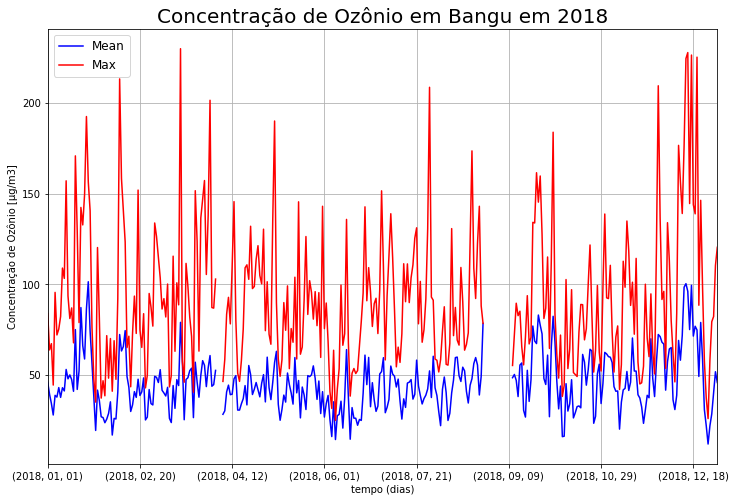
\includegraphics[width=\linewidth]{img/graphic4.png}
    \caption{Concentração de Ozônio em 2018.}
    \label{time-series}
\end{figure}

\subsection{Autocorrelação}

Precisamos encontrar padrões na série temporal, a fim de encontrar possíveis
tendências, não necessariamente lineares, sazonalidades ou mudanças cíclicas. Para
isso, utilizo uma medida de relação linear entre valores com atraso da série.
Definimos $r_k$ como essa medida entre os valores $y_t$ e $y_{t - k}$, para
todos os valores de $y_t$ capturados. Esse método é derivado da correlação de
Pearson. 

\begin{equation}
    \label{autocorrelation}
    r_k = \frac{\sum_{t = k + 1}^T (y_t - \overline{y})(y_{t - k} -
    \overline{y})}{\sum_{k=1}^T (y_t - \overline{y})^2}    
\end{equation}

A partir disso, é possível gerar a função de autocorrelação. Neste trabalho,
explorei essa função em relação aos meses e às horas. Em relação aos meses, meu
$k$ varia entre os valores de $0$ a $12$. De fato $r_0 = 1$. Espera-se que a
autocorrelação seja zero se o tempo não tenha influência sobre os dados. Nesse
caso, chamamos a série de ruído branco. Claro que como o conjunto de dados tem
tamanho finito, a autocorrelação dificilmente será $0$. Desta maneira, para
esses casos, é esperado que os valores estejam entre os limites $\pm
\frac{2}{\sqrt{T}}$ com probabilidade $95\%$, onde $T$ é o tamanho da amostra.
A figura \ref{acf-months} representa a função. Note o quão insignificantes se
tornam os limites. 

Valores altos para pequenos atrasos indicam tendência na série, já que
existe uma correlação alta entre os valores de um mês com os valores do mês
anterior. Entretanto, como o decréscimo não é suave, a tendência não é tão
observada. Também é interessante observar o efeito da sazonalidade em períodos
de 6 meses. Isso pode estar relacionado a período mais quente e frio, e a
alternância, nesses casos, da concentração de ozônio. 

No caso das horas, também foi observada alta correlação para valores de
atraso pequenos, mas o resultado foi pouco elucidativo. 

\begin{figure}  
    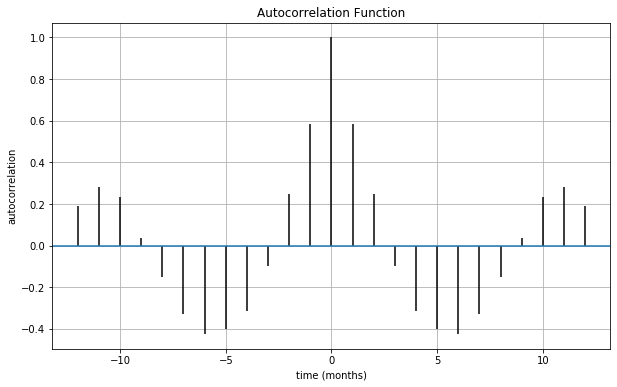
\includegraphics[width=\linewidth]{img/graphic3.png}
    \caption{Função de autocorrelação em relação aos meses. As linhas azuis
    representam os limites. }
    \label{acf-months}
\end{figure}

\subsection{Estacionariedade}

Uma série é dita estacionária quando ao passar do tempo, seus valores
mantem-se ao redor da média e variância constante. Quando uma série apresenta
tendência, ela não é estacionária. A importância de uma série estacionária é
para a realização do modelo, já que vários deles são descritos sobre séries
estacionárias. Para testar se nossa série temporal é estacionária,
consideremos o teste Dickey-Fuller Aumentado, um tipo de teste de uma raíz,
uma causa para a não estacionariedade.

$$H_0 : ~there~is~unit~root~(non~stationary)$$
$$H_1 : ~there~is~no~unit~root~(stationary)$$

Considero o nível de significância de 5\%. O p-valor do teste esteve na ordem
de $10^{-30}$, e a hipótese nula foi rejeitada. O teste foi realizado em
Python, através da função \textit{adfuller} do módulo para análide de séries
temporais \textit{statsmodels.tsa}. Para esse teste em Python, conferir
\cite{adf-test}. Outro fator importante de se analisar é a ergodicidade,
porém, nesse ensaio, assumirei a série como engórdica. 

\section{Modelando Séries Temporais}

Para modelar uma série temporal, a fim de fazer futuras predições, existem
diversos métodos apresentados pela literatura. Os dados consideram as máxima
média a cada 8h, que são consideradas para o cálculo do IQA no banco de dados.
Para os valores faltantes, preenchi com o valor anterior e deixo para futuros
trabalhos estudar métodos mais eficazes. Os dados não são afetados de forma
significativa por inflação, mudança na população ou calendário, pois o
intervalo temporal em anos não é muito grande. 

Para realizar os seguintes métodos, desenvolvo um processo para a análise do
resultado com o diagnóstico dos dos resíduos através do teste para
autocorrelação de \textit{Portmanteau}. Nesse teste, testamos se as primeiras $h$
autocorrelações são significantemente diferentes da esperada em ruído branco.
Existem várias estatísticas para esse teste, como, por exemplo, o teste
\textit{Box-Pierce} e, mais preciso, o teste \textit{Ljung-Box}, conforme
apêndice A. 

Para avaliar a precisão de nossas previsões, utilizo o método de
Cross-Validation para dividir os dados, mais de uma vez, em treino e teste. Ao
fim, para cada divisão temporal, calculo a precisão do modelo através do
método da Média Absoluta de Erros de Escala (Veja apêndice B) e, depois, faço
a média desse cálculo de previsão. 

\textbf{Métodos Estudados nesse trabalho: }
\begin{enumerate}
    \item Método da Média;
    \item Regressão Linear;
    \item Suavização Exponencial; 
\end{enumerate}

\subsection{Método da Média}

Nesse método de previsão, o modelo simplesmente afirma que a próxima
observação é a média das observações anteriores. Ele tem sua importância para
teste de sanidade e verificação dos métodos de análise de resultado.

\subsection{Regressão Linear}

A regressão linear admite que exista uma relação linear entre duas ou mais
séries temporais. Assim, 
$$y_t = \beta_0 + \beta_1x_{1,t} + ... + \beta_nx_{n,t}+ \epsilon_t$$
A variável $\epsilon$ captura tudo que as variáveis escolhidas não capturam.
Observe que os parâmetros indicam o quanto as variáveis são relacionadas e
como elas se relacionam (positivamente ou negativamente). Assumimos algumas
coisas sobre os erros: 

\begin{itemize}
    \item A média $0$;
    \item São não autocorrelacionados. Caso não fossem, existiria informação
    adicional que não foi extraída dos dados;
    \item São não relacionados com as variáveis preditoras, que representam as
    variáveis $x_{i,t}$. 
    \item É interessante, mas não necessário, que os erros sejam normalmente
    distribuídos. 
\end{itemize}

O método que utilizo para escolher os parâmetros é a estimação de mínimos
quadrados. Também, para esse modelo, lanço mão do coefieciente de
determinação, o $R^2$ (Veja Apêncice C).

As variáveis que utilizarei para esse modelo são Temperatura, Radiação Solar, 
Velocidade do Vento e Umidade Relativa. Essas quatro variáveis apresentam os
maiores valores absolutos de correlação e tem relação direta com a formação do
ozônio. A radiação solar, é um exemplo já construído na literatura e tem
relação direta com o ozônio \cite{solarRadiation}. 

Além disso, eu crio 11 variáveis indicadoras para os meses, a fim de capturar
a sazonalidade ou tendências em certos períodos. É importante dizer que não é 
necessária mais uma variável, pois ela estará incluída no parâmetro de
interceptação, que não acompanha variáveis independentes. Ao colocar essa
variável, podemos criar uma \textit{variável indicadora armadilha}. Essas
variáveis indicam $1$ para o mês correspondente e $0$ caso contrário. 

\subsection{Suavização Exponencial}

Proposta no final dos anos de 1950, por Brown, Holt e Winters, a suavização
exponenicial tem motivado diversos sucessos em previsões. Basicamente, esse
método faz uma média ponderada das observações passadas, só que esses pesos
decaem exponencialmente com o tempo. Especificamente, os pesos decrescem com
uma razão geométrica. Nesse método, existem diversas variações. Chamamos de
Suavização Exponencial Simples a seguinte equação:

$$\hat{y}_{T+1|T} = \sum_{j=0}^{T-1} \alpha(1 - \alpha)^jy_{T-j} + (1-
\alpha)l_0,$$
onde, os parâmetros $\alpha$ e $l_0$ devem ser estimados. $l_0$ a primeira
estimação, enquanto $\alpha$ é um valor entre $0$ e $1$ que indica o quando de
importância se dá aos eventos passados. 

Entretanto, nesse trabalho, desenvolvo um modelo para capturar a sazonalidade
dos dados, onde existe a equação de previsão e três equações de suavização: o
componente de tendência, o componente sazonal e o nível da suavização. Nesse
caso, existem mais dois parâmetros a serem estimados, além de um parâmetro de
sazonalidade que indica o número de períodos do ano. Esse modelo foi
desenvolvido por Holt e Winters. 

A fim de encontrar os parâmetros, também utilizo o método de minimização de
quadrados dos erros. 